% Chapter Template

\chapter{Thermoregulation in gregarious Dipteran larvae: evidence of species-specific temperature selection}

\label{Chapter5}

\lhead{Chapitre 5. \emph{Thermoregulation in gregarious Dipteran larvae: evidence of species-specific temperature selection }} 

Cindy \textsc{Aubernon}\up{a}, Julien \textsc{Boulay}\up{a,b}, Valéry \textsc{Hédouin}\up{a} and Damien \textsc{Charabidzé}\up{a}

\up{a} Univ. Lille, CHU Lille, EA 7367 - UTML - Unité de Taphonomie Médico-Légale, Lille, France\\
\up{b} Université Libre de Bruxelles, Unit of Social Ecology, Brussels, Belgium\\


Article soumis à \emph{Entomologia Experimentalis et Applicata}.

\cleardoublepage
%----------------------------------------------------------------------------------------
%	SECTION 1
%----------------------------------------------------------------------------------------
	\section{Abstract}
There is a clear recognition that local temperature controls the development time of blowfly larvae (Diptera Calliphoridae). In this context, it has been supposed that each species has an optimal development temperature characterized by a short development time and high survival rate. Accordingly, the temperature felt by larvae during their development on a corpse appears to be strongly dependent on behavioural regulation. We hypothesized that the temperature selected by larvae may not only minimize their development time on the cadaver but also may result from a trade-off between development quality and duration. According to this hypothesis, larvae of each species should select the warmest temperature that allows them to develop normally. Consequently, the use of ambient temperature or maximum maggot-mass temperature to estimate the development time of larvae on a corpse would be meaningless.
We designed the Thermograde, which is an 80 cm long linear thermal gradient setup, to determine species-specific preferential temperatures. This experiment was performed using 3 different species: \textit{Lucilia sericata} (Meigen, 1826), \textit{Calliphora vomitoria} (Robineau-Desvoidy, 1830) and \textit{Calliphora vicina} (Linnaeus, 1758). Eighty young third instars were homogeneously placed on the Thermograde along with 500 g of mixed beef liver. The location of larvae in the thermal gradient was observed after 19 h. Fifteen replications were performed for each species. The larvae formed masses that were always located at the same species-specific temperatures, which were 33.3$\pm$1.52\up{o}C for \textit{L. sericata}, 29.61$\pm$1.63\up{o}C for \textit{C. vomitoria} and 22.43$\pm$1.55\up{o}C for \textit{C. vicina}. These innovative results reveal for the first time important information concerning larval displacement and thermoregulation strategies. Our experiments raise questions regarding the way larvae moved on the gradient and located their preferential temperatures. Further studies need to be conducted on individual larva displacement and thermoregulation strategies, which are also important for Post-Mortem Interval (PMI) estimation in forensic entomology. 

\textit{Keywords:} \textit{Calliphora vicina} - \textit{Calliphora vomitoria} - Calliphoridae - collective choice - develoment time - forensic entomology - \textit{Lucilia sericata} - trade-off.

\clearpage

%----------------------------------------------------------------------------------------
%	SECTION 2
%----------------------------------------------------------------------------------------
	\section{Introduction}
Necrophagous blowfly larvae (Diptera Calliphoridae) feed on decomposing remains, mostly on vertebrate cadavers \cite{szpila_key_2009}. Like all poikilothermic species, the internal temperature of larvae depends on the environmental temperature \cite{chapman_insects:_1998}; in other words, their physiological processes are directly controlled by external heat. This is especially true for development speed, which is directly linked to local temperature. Developmental curves generally show a sigmoidal relationship: the development rate is close to zero at low values, increases linearly over a medium range of temperatures, and then slows down at higher temperatures until reaching a lethal point \cite{dent_quantifying_1997}. For necrophagous blowflies, the relationship between temperature and development time has been well-documented in the context of forensic entomology \citep{grassberger_effect_2001,swiger_effects_2007}. Restricting the development-time of necrophagous larvae on the cadaver seems to be essential to prevent food shortages because of the ephemeral duration of animal carcasses in the field \cite{payne_summer_1965}. Furthermore, because the probability of being predated or parasitized increases along with feeding duration on the cadaver, faster development should limit predation or parasitism and increase the larval survival rate \cite{roe_development_2015}. Accordingly, we theorized that larvae would prefer temperatures that speed up their development, thus minimizing the time they must spend on the carcass.  

Various thermoregulation behaviours exist among insects. Because of their poikilothermic physiology, insects select and move between specific micro-climates to adapt their body temperatures \cite{may_insect_1979}. For necrophagous larvae, a preferential choice for warm areas was reported for larvae growing on carcasses that had both sunny and shady sides \cite{sharanowski_insect_2008}. Conversely, larval escape from too-hot locations was also observed \citep{richards_thermal_2009,charabidze_larval-mass_2011}. 

This study was designed 1) to test the ability of necrophagous larvae to orientate in a heterogeneous thermal environment and 2) to compare the temperatures selected by the larvae of 3 common blowfly species. For this purpose, we designed an original setup we named Thermograde. This setup consists of a food-supplied linear thermal gradient that allows larvae to move, feed and grow in close-to-real conditions and to choose to stay and feed at a given temperature (i.e., a location in the Thermograde). Three common species of forensic importance were tested using this setup: \textit{Lucilia sericata} (Meigen, 1826), \textit{Calliphora vicina} (Robineau-Desvoidy, 1830) and \textit{Calliphora vomitoria} (Linnaeus, 1758). 

%----------------------------------------------------------------------------------------
%	SECTION 3
%----------------------------------------------------------------------------------------
	\section{Materials and methods}  
%-----------------------
%	SUBSECTION 1
%----------------------    
    
    	\subsection{Thermograde}
Larvae of three Diptera Calliphoridae species were used in this study; \textit{Lucilia sericata}, \textit{Calliphora vomitoria} and \textit{Calliphora vicina}. The first two strains originated from the north of France, while the \textit{C. vicina} strain originated from Belgium. Insects were reared in tulle cages (50x50x50 cm). Inbreeding was controlled by introducing 50$\%$ wild-type individuals. Adult flies (250$\pm$100) from a single emergence pool were maintained at 20$\pm$2\up{o}C with a daylight photoperiod and for a maximum of 30 days. Flies were fed \textit{ad libitum} with caster sugar and water. To allow egg-laying, 20$\pm$5 g of mixed beef liver was placed in a pill-box inside the insectariums. After egg-laying, the eggs were removed and placed at 19\up{o}C in a climatic chamber (SANYO MIR, 554) in closed plastic boxes (143x105x59 mm) with 100$\pm$5 g of mixed beef liver until reaching the third instar. Corresponding development times for each species at 19\up{o}C were found on the ForenSeek database (https://www.forenseek.org) \citep{greenberg_flies_1991,grassberger_effect_2001,greenberg_different_1993}.

Experiments were performed under controlled conditions using the Thermograde, an apparatus we designed to provide a linear thermal gradient (Figures \ref{fig:thermo1} and \ref{fig:thermo2}). The Thermograde is composed of a heating shelf and a gutter-like galvanized steel bar (5x5x80 cm). Fresh mixed beef liver (500 g) was spread inside the bar to create a 2 cm high food layer. The heating shelf was placed underneath the bar to spread the heat along the bar and obtain a linear thermal gradient inside the beef liver. The shape of this gradient was controlled by changing ambient (i.e., outside the bar) temperature. I-button temperature recorders (DS1921G Thermochron i-Button, $\pm$0.5\up{o}C) were placed every 5 cm (from 2.5 to 77.5 cm) to monitor the local temperature.

For each experiment, 80 young third instars were sampled from the rearing box and starved in a pill-box for 4 hours at 19\up{o}C \cite{charabidze_discontinuous_2013}. This number of insects was previously shown to be sufficient to allow aggregation \cite{boulay_evidence_2013} yet small enough to prevent larval-mass effect and thus heat emission \citep{charabidze_larval-mass_2011,heaton_quantifying_2014}. After starvation, larvae were spread on the beef liver inside the bar in a homogeneous manner (one larva every centimetre). Finally, the bar was closed with an opaque black plastic cap (5.5x3x80 cm).

Experiments were stopped after 19 hours; according to developmental data for the 3 species, this duration was short enough to prevent larvae reaching the wandering stage \citep{greenberg_flies_1991,greenberg_different_1993,grassberger_effect_2001}. The cover was removed, and the Thermograde was divided into 5 cm sections. The beef liver inside each section was removed, and the larvae inside were counted. The temperature values recorded during the experiment were extracted from the temperature recorders. Fifteen replicates were performed for each species.

In addition, 2 control experiments were performed on \textit{L. sericata}. The first control experiment used the Thermograde without heating (Control 1) (i.e., homogeneous temperature, 20$\pm$1\up{o}C) to test the distribution of the larvae inside the Thermograde (6 replications). The second control (Control 2) was designed to ensure that heating had not affected the beef liver’s nutritional value \cite{rice_effects_1953}. Indeed, it can be supposed that larvae might select a given heated area according to the effect of temperature on the nutrient quality of food. For this purpose, 'cooked' liver (37\up{o}C over 19 h) was used instead of fresh beef liver to create the thermal gradient. By doing this, we obtained the same thermal gradient created during the regular (non-control) experiments, but with previously heat-exposed meat. Fifteen replications were performed.

\begin{figure}[ht]
\centering
		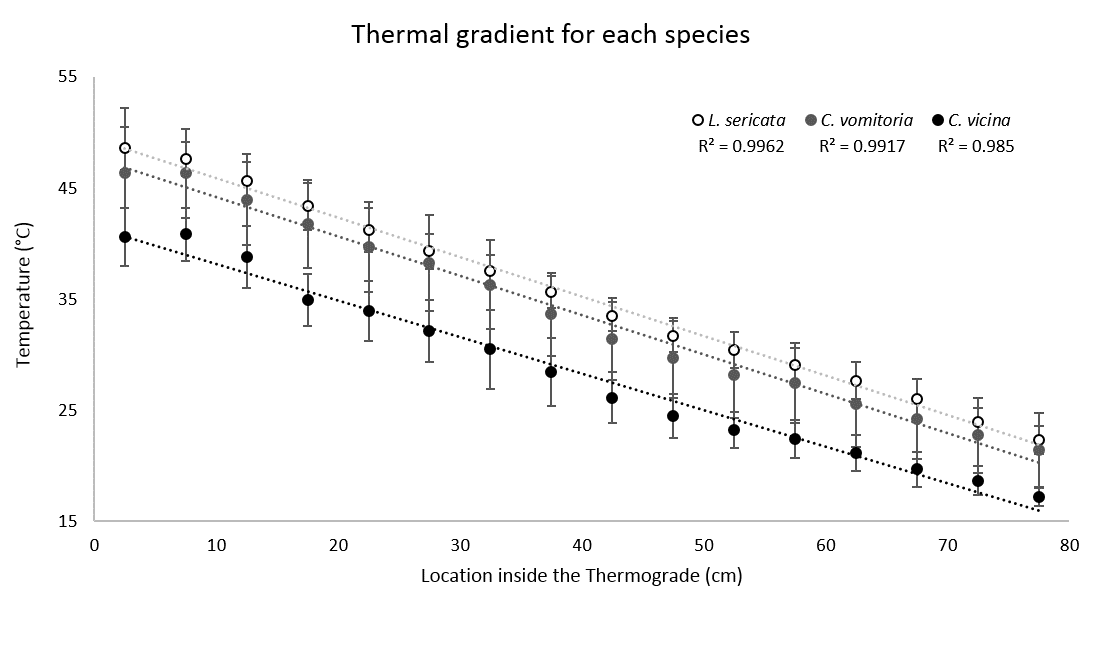
\includegraphics[width=1 \textwidth]{Figures/thermograde1.png}
		\rule{35em}{0.5pt}
		\caption[Thermo1]{The 3 thermal gradients used to test thermal preferences of the species. Points represent the mean temperature ($\pm$SD) inside the food substrate (beef liver) according to their locations inside the Thermograde and the species studied \\(N=15 for each species).}
	\label{fig:thermo1}
\end{figure}

\begin{figure}[ht]
\centering
		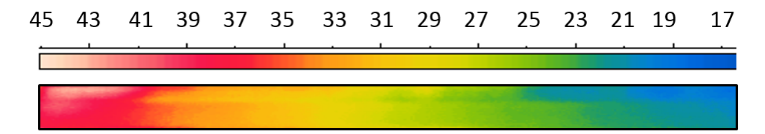
\includegraphics[width=0.9 \textwidth]{Figures/thermograde2.png}
		\rule{35em}{0.5pt}
		\caption[Thermo2]{Thermic photography of the Thermograde for \textit{L. sericata} in Celcius \\degrees (Camera FLIR T425, 320x240 pixels).}
	\label{fig:thermo2}
\end{figure}    
    
%-----------------------
%	SUBSECTION 2
%----------------------    
    
    	\subsection{Binary choice} 
The purpose of this experiment was to test whether the larvae in the Thermograde selected an area based on local temperature or because of food quality resulting from heating. 

The setup was composed of two translucent pill-boxes (150 ml, diam. x h: 57x73 mm) closed with a screw cap drilled with 1 mm holes and connected with a 40 mm long translucent plastic pipe (Figure \ref{fig:setupcindy}). Forty grams of unfrozen beef liver, previously heated for 19 hours at either 33\up{o}C or 37\up{o}C, were placed in each pill-box. The quantity of food in the pill-boxes was selected to expect a 100$\%$ survival rate according to Ireland and Turner \cite{ireland_effects_2006}. Twenty larvae previously starved for 4 h at 19\up{o}C \cite{charabidze_discontinuous_2013} were deposited inside each of these two pill-boxes for a total of 40 larvae per setup. The entire setup was placed in a climatic chamber (SANYO MIR, 554) at 19\up{o}C for 19 h. The pill-boxes and tube were then disassembled, and the larvae inside each of the 3 compartments (the right and left pill-boxes and the tube) were counted. The setup was kept at 19\up{o}C during all experiments, but the liver was heated to varying temperatures before the experiments began. Three liver-temperature conditions were tested: 33\up{o}C vs. 33\up{o}C (i.e., 33\up{o}C control, N=15), 37\up{o}C vs. 37\up{o}C (i.e., 37\up{o}C control, N=15) and 33\up{o}C vs. 37\up{o}C (N=15). 

\begin{figure}[ht]
\centering
		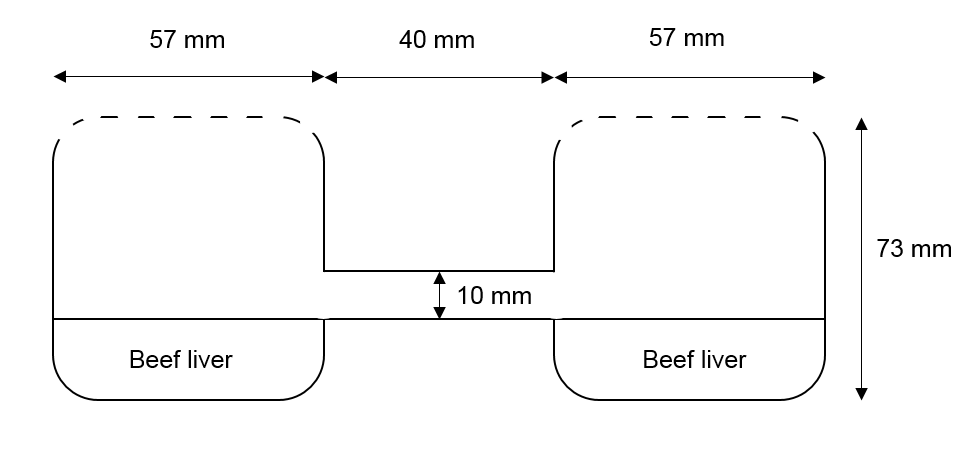
\includegraphics[width=0.9 \textwidth]{Figures/setupbinarycindy.png}
		\rule{35em}{0.5pt}
		\caption[SetupCindy]{Scheme of the binary-choice setup. Beef liver was heated at 33\up{o}C or 37\up{o}C for 19 h before experiments. After the beef liver had cooled to 19\up{o}C, twenty \textit{L. sericata} larvae were placed in each side, and the setup was kept at 19\up{o}C for 19 hours.}
	\label{fig:setupcindy}
\end{figure}    
        
%-----------------------
%	SUBSECTION 3
%----------------------    
    
    	\subsection{Statistical analysis} 
Statistical tests with a significance threshold at 0.05 were used to analyse the results, using XLStat (Addinsoft) software. A chi-square test was used for the larval distribution, and Fisher’s test was used for the distribution of the aggregates. A Shapiro-Wilk’s test and a Bartlett’s test were performed to analyse the mean selected temperature’s distribution and homoscedasticity. An ANOVA and post-hoc Tukey’s and Dunnett’s tests were performed to compare the mean survival rate and the mean selected temperature between species. Finally, a z test was performed to analyse binary choice for each replication, and Student’s t-test was used to compare the mean number of individuals.


%----------------------------------------------------------------------------------------
%	SECTION 4
%----------------------------------------------------------------------------------------
	\section{Results}  
Our setup was designed to allow larval thermal choice under non-stressing rearing conditions. The repartition of \textit{L. sericata} larvae in the Control 1 condition significantly differed from a homogeneous distribution (X\up{2} test: p<0.0001). During each replication, most larvae were observed aggregated together in a single mass. The location of this mass in the setup differed between replicates, but did not statistically differ to a random location (Fisher's test: p=0.82). In other words, without heating (i.e., homogeneous temperature), larvae aggregated together inside the Thermograde, but the location of the aggregate varied between experiments and was not preferentially located in a given area (Figure \ref{fig:percentcindy}). 
When heating was turned on, the thermal gradient inside the Thermograde was close to linear, with a loss of temperature equal to 1.77\up{o}C, 1.77\up{o}C and 1.65\up{o}C per centimeter for, respectively, \textit{L. sericata}, \textit{C. vomitoria} and \textit{C. vicina} (Figure \ref{fig:thermo1}). 

\begin{figure}[ht]
\centering
		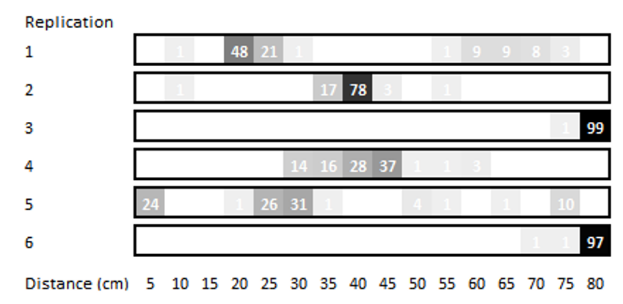
\includegraphics[width=0.9 \textwidth]{Figures/percentcindy.png}
		\rule{35em}{0.5pt}
		\caption[PercentCindy]{Percentage of larvae in each section of the Thermograde according to replication (Control 1). In pale gray, low density of larvae, in dark, high density.}
	\label{fig:percentcindy}
\end{figure}    

Only a few larvae died during experiments. The mean survival rate was 78.42$\pm$14.41$\%$ for \textit{L. sericata}, 87.33$\pm$9.40$\%$ for \textit{C. vomitoria} and 87$\pm$6.57 for \textit{C. vicina}. No difference existed between the survival rates of the tested species and the \textit{L. sericata} survival rate in Control 2 (ANOVA: F=2.12, p=0.11; Tukey’s procedure: \textit{L. sericata} vs. \textit{C. vomitoria}: p=0.16, \textit{L. sericata} vs. \textit{C. vicina}: p=0.14, \textit{C. vomitoria} vs. \textit{C. vicina}: p=1).

The results showed that \textit{L. sericata}, \textit{C. vomitoria} and \textit{C. vicina’s} aggregates (X\up{2} test: p<0.0001) were not randomly located on the thermal gradient (Fisher’s test: \textit{L. sericata}: p=0.01; \textit{C. vomitoria}: p=0.002, \textit{C. vicina}: p<0.0001). Larvae of each species were preferentially observed in a species-specific location corresponding to a given temperature (Figure \ref{fig:boxplotcindy}). \textit{L. sericata} larvae were found located at 33.3$\pm$1.52\up{o}C while \textit{C. vomitoria} larvae were found at 29.61$\pm$1.63\up{o}C and \textit{C. vicina} larvae at 22.58$\pm$1.55\up{o}C. These temperature values differed significantly between the 3 species (ANOVA: F=144.60, p<0.0001; Tukey’s procedure: \textit{L. sericata} vs. \textit{C. vomitoria}: p<0.0001, \textit{L. sericata} vs. \textit{C. vicina}: p<0.0001, \textit{C. vomitoria} vs. \textit{C. vicina}: p=0.0001). 

\begin{figure}[ht]
\centering
		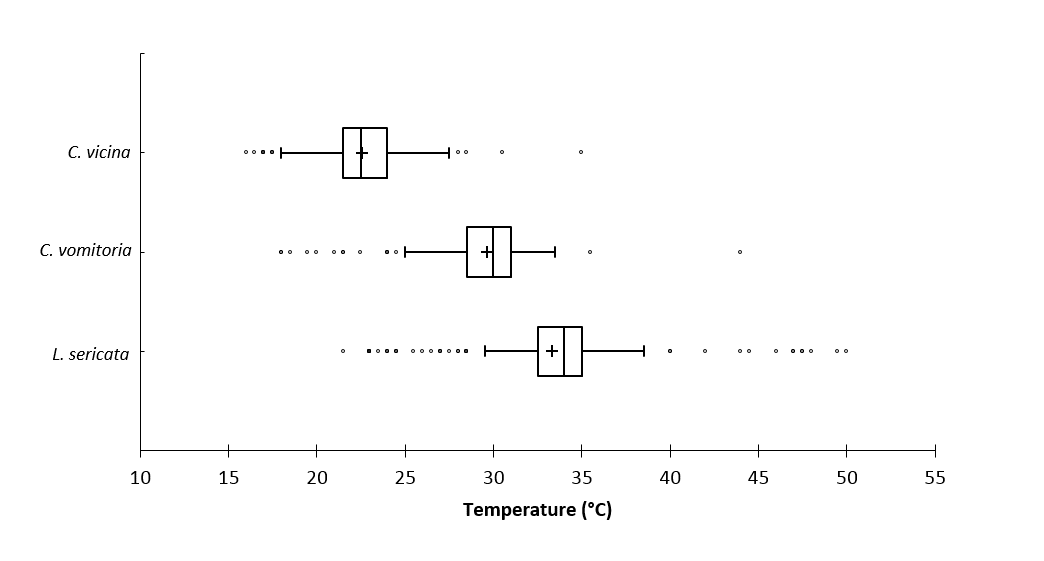
\includegraphics[width=1 \textwidth]{Figures/boxplotcindy.png}
		\rule{35em}{0.5pt}
		\caption[BoxplotCindy]{Box plots representing the location of the larvae according to the temperature gradient inside the Thermograde. The vertical bar inside the box represents the median, the cross represents the mean, and the dots represent outliers, i.e., isolated individuals not located in the aggregate.}
	\label{fig:boxplotcindy}
\end{figure}   

The larval distributions were normal (Shapiro-Wilk’s test: \textit{L. sericata}: W=0.96, p=0.45; \textit{C. vomitoria}: W=0.96, p=0.287; \textit{C. vicina}: W=0.96, p=0.45), and the variance around the mean did not differ according to species (Bartlett’s test: p=0.88) (Figure \ref{fig:districindy}).


\begin{figure}[ht]
\centering
		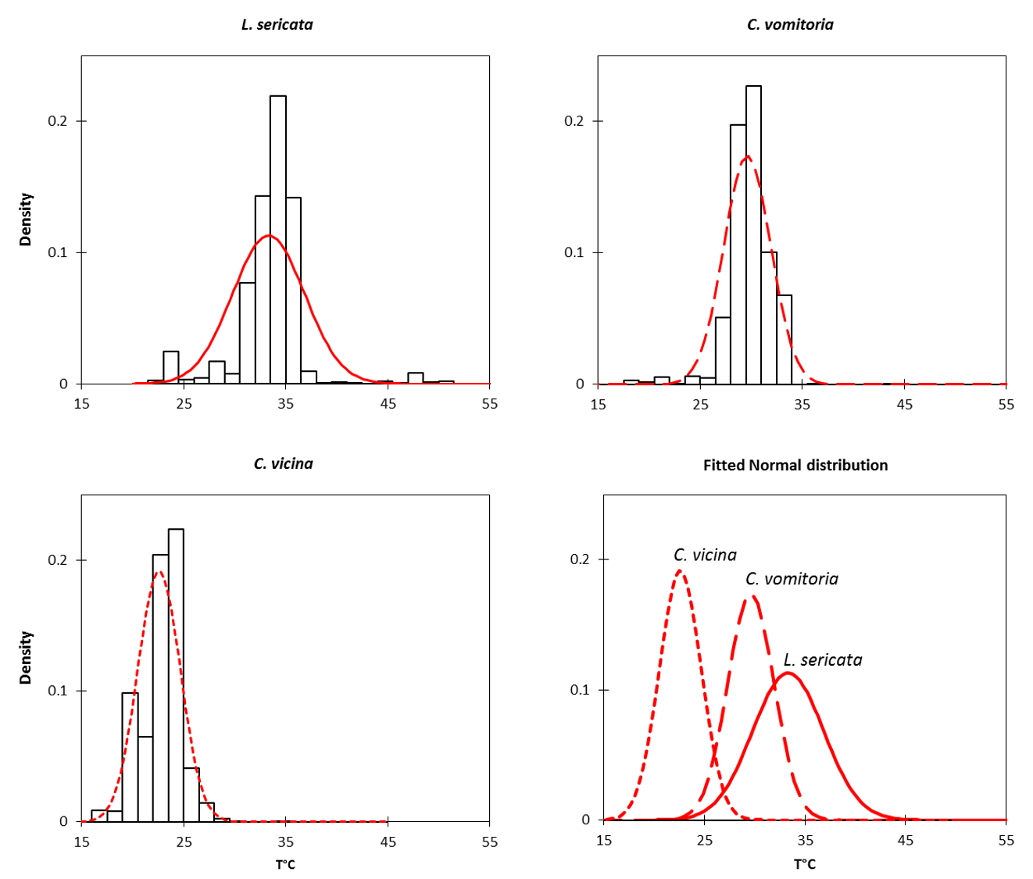
\includegraphics[width=1 \textwidth]{Figures/districindy.png}
		\rule{35em}{0.5pt}
		\caption[DistriCindy]{Distributions of larvae as density inside the Thermograde for each species according to temperature.}
	\label{fig:districindy}
\end{figure}  



Finally, the repartition of \textit{L. sericata} larvae in Control 2 differed significantly from a homogeneous distribution (X\up{2} test: p<0.0001). Larvae were observed aggregated at a mean temperature of 33$\pm$1.56\up{o}C (Fisher’s test: p=0.01), which was not different from \textit{L. sericata}’s selected temperature during the raw meat experiments (Dunnett’s procedure: p=0.91). Last, we observed a survival rate of 83.25$\pm$6.88$\%$, which was also no different from the raw meat experiments (Dunnett’s procedure: p=0.65). 

Each replicate was divided into one 'winner' pill-box (the one with more larvae inside) and one 'loser' pill-box (Figure \ref{fig:percent2cindy}). We determined the winner and loser pill-boxes according to the number of individuals in each pill-box for each replication by comparing the single proportion with a z test. Three replications (out of 15) were not significant for the 33\up{o}C control, four for the 37\up{o}C control and four 33 vs. 37\up{o}C experiments. These not-significant choices were removed from statistical analysis.

\begin{figure}[ht]
\centering
		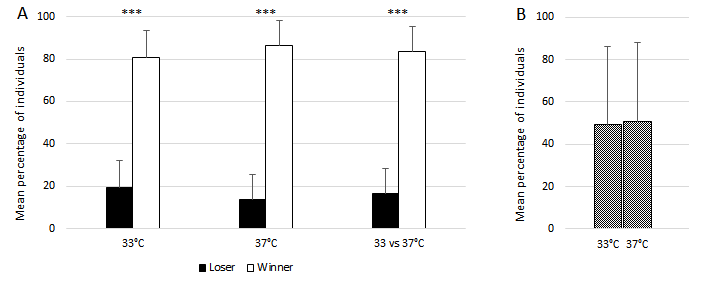
\includegraphics[width=1 \textwidth]{Figures/percent2cindy.png}
		\rule{35em}{0.5pt}
		\caption[Percent2Cindy]{Mean percentage of individuals ($\pm$SD) according to experimental conditions. \textbf{A}. Controls (33 vs. 33 and 37 vs. 37) and experiment (33 vs. 37) facing winner (white) and loser (black) pill box.  \textbf{B}. 33 vs. 37\up{o}C.}
	\label{fig:percent2cindy}
\end{figure}  

In the 33\up{o}C control, the 37\up{o}C control and the 33 vs. 37\up{o}C experiments, we noticed that the mean percentage of individuals was higher in winner pill-boxes, with 80.59$\%$ vs. 19.41$\%$ for 33\up{o}C control (Student’s test: p<0.0001), 86.21$\%$ vs. 13.79$\%$ for 37\up{o}C control (Student’s test: p<0.0001) and 83.58$\%$ vs. 16.42$\%$ for 33 vs. 37\up{o}C experiment. Finally, we noticed that for the 33 vs. 37\up{o}C experiment, the 33\up{o}C pill-box won 49.12$\%$ of the time, while the 37\up{o}C pill-box won 50.88$\%$ of the time — that is, 33\up{o}C was the winner 5 times and 37\up{o}C was the winner 6 times. This did not differ from an equal (fifty-fifty) repartition (z test: p=0.76; X\up{2} test: p=0.90). Last, the mean percentage of individuals was the same in both 33\up{o}C and 37\up{o}C pill-boxes (Student’s test: p=0.939) and did not show larval preference for a given food substrate.
        
  
%----------------------------------------------------------------------------------------
%	SECTION 5
%----------------------------------------------------------------------------------------
	\section{Discussion}    
  
This study is the first observation of collective preferential temperature selection by 3 species of necrophagous larvae of forensic importance. The highlight of this study was that the larvae of each species were able to locate and select a preferred species-specific temperature. These values were 33.3$\pm$1.52\up{o}C for \textit{L. sericata}, 29.6$\pm$1.63\up{o}C for \textit{C. vomitoria} and 22.43$\pm$1.55\up{o}C for \textit{C. vicina}. Such a clear result raises interesting questions regarding developmental physiology and trade-off selection in necrophagous larvae.

It is known from the literature that a measurable increase in temperature can arise inside aggregates (larval-mass effect) \citep{slone_thermoregulation_2007,charabidze_larval-mass_2011}. Such local heating begins with an aggregate of approximately 1000 third instar individuals and increases with the quantity of larvae \cite{heaton_quantifying_2014}. During our experiments, the number of larvae was kept low enough to prevent this phenomenon, and thermometers inside the bar did not record any local increase of temperature in the places where larvae were aggregated. Accordingly, any maggot-mass effect in our experiment can be excluded. One might also object that the larvae did not select a given temperature but instead selected a food quality. According to this view, the nutritional value of the beef liver should change depending on its temperature and according to species. However, considering \textit{L. sericata}, no preference was observed between experiments with raw or 37\up{o}C-incubated food (Control 2). Furthermore, binary-choice test experiments did not show any larval preference between 33\up{o}C- or 37\up{o}C-incubated food; larvae were gathered at both temperatures and at the same mean percentage. We concluded from these experiments that larval distribution in the Thermograde was due not to differences in food quality, but to preferential temperature selection.

Larvae were able to aggregate and gather themselves into a single group inside the Thermograde \citep{rivers_physiological_2011,boulay_evidence_2013}. Under Control 1’s conditions (20$\pm$1\up{o}C homogeneous temperature, no heating), these aggregates were located randomly throughout the apparatus. This control demonstrates that the distributions observed in the gradient experiments were not due to setup bias or increased probability to cross and aggregate in the middle of the Thermograde. On the contrary, for the 3 tested species, aggregates clearly occurred in different areas of the Thermograde at given species-specific temperature values. In addition to the well-known larval aggregation behaviour \cite{boulay_evidence_2013}, our results demonstrate for the first time the search and collective choice behaviour of necrophagous larvae for a given temperature. A key point is that this temperature differed between the three studied species; the selected temperature was highly species-specific. Indeed, while \textit{L. sericata} larvae were always found strongly grouped at approximately 33.3$\pm$1.52\up{o}C, \textit{C. vomitoria} larvae aggregated in the 29.61$\pm$1.63\up{o}C part of the Thermograde, and \textit{C. vicina} larvae were found located at 22.43$\pm$1.55\up{o}C.
        
In a recent study, \citet{johnson_tracking_2014} studied larval temperature selection of two necrophagous species, \textit{C. vicina} and \textit{Chrysomya rufifacies} (Macquart, 1842). Using a thermal gradient created with a heating spot and a cold bath, the authors observed three times the selection of third instar larvae placed in the setup. The larval-selected temperature was defined as the value where larvae stopped and stayed after 2 hours; the temperature at this point was then measured. According to this protocol, \citet{johnson_tracking_2014} observed that \textit{C. vicina} larvae selected 'temperature approximately 24.5\up{o}C'. This value is 2\up{o}C above the one we measured (22.43\up{o}C). This difference may be explained by the few replicates performed (only 3 with 3\up{rd} instar), the exactness of the thermal gradient used (the temperature was known each 10 cm in a range of 23\up{o}C to 54\up{o}C) or by differences between the two studied insect populations. Indeed, the \textit{Calliphora vicina} larvae studied by \citet{johnson_tracking_2014} came from Australia, while those used for this study came from Belgium. It is known from the literature that local fly populations are morphologically and physiologically adapted to their environment \citep{donovan_larval_2006,lebouvier_significance_2011,tarone_population_2011}. For example, differences exist in the diapause and low-temperature survival rates between Scottish, Finnish and Italian populations of \textit{C. vicina} \cite{saunders_effects_2013}. \textit{C. vicina} from Switzerland have even been shown to develop in extremely cold environments that are usually not suitable for this species \cite{faucherre_behavior_1999}.     

The reasons behind the temperature choices by each species are still unknown. Larvae feeding and growing on carrion face high selection pressure \cite{campobasso_factors_2001}. This is noticeably true during feeding stages; decomposition processes can alter flesh within a few days, and quick drying of the tissues can make cadavers inedible for blowfly larvae \cite{clark_postmortem_1997}. Last but not least, numerous opportunistic scavengers, such as wild boars, foxes or crows, can eat small cadavers or deflesh larger ones in a few minutes \cite{haglund_dog_1997}. Bearing this in mind, it appears that larvae should tend to minimize their development duration and thus the time spent on the cadaver. This can be achieved by individuals moving to high-temperature areas and thus increasing their development rate \cite{grassberger_effect_2001}. According to this assumption, larvae of each species should select the warmest temperature allowing their development. However, developmental data currently available from the literature do not validate this hypothesis. Indeed, published developmental data are mostly restricted to low- or medium-temperature ranges; only a few values are available for high temperature. \citet{reiter_growth_1984} noticed that when constant temperatures were beyond 30\up{o}C, \textit{C. vicina} larvae were deformed and or died. \citet{donovan_larval_2006} reported a larval lethal temperature for \textit{C. vicina} of 35\up{o}C, more than 10\up{o}C above the value larvae selected in the Thermograde. However, we hypothesized that the temperature preferred by larvae would not be selected solely to minimize development time on the cadaver, but instead may result from a trade-off between development quality and duration. Indeed, temperature controls not only the physiology of the larvae and their development rate \cite{chapman_insects:_1998} but also the quality of their growth and thus their fitness. Larvae growing under too-warm temperatures could be malformed or too small \cite{reiter_growth_1984}, and physiological parameters, such as respiration or eggs, may also be impacted \cite{williams_growth_1984}. Such effects are even transmitted to the second generation: \citet{zamudio_bigger_1995} demonstrated that \textit{Drosophila melanogaster} (Meigen, 1830) fitness depends on parental rearing temperature. Detailed developmental data (duration, survival rate, length and weight) at high temperature would thus be necessary to verify our developmental trade-off hypothesis; breeding experiments are currently being performed in our laboratory to gather developmental data at high temperature for the 3 species targeted by this study.

Finally, our experiments raise questions regarding the way larvae moved on the gradient and located their preferential temperature. From our results, it is not possible to determine whether the aggregate was created by the sum of individual thermal preferences, or whether larvae first aggregate and then move together. Previous studies of maggot masses noticed a turnover of larvae inside masses, a behaviour that supposedly allows larvae cooling and prevents overheating of the aggregates \citep{charabidze_discontinuous_2013,rivers_heat_2015}. Further studies need to be conducted on individual larvae displacement and thermoregulation strategies, which are also important for post-mortem interval (PMI) estimation in forensic entomology. 

%----------------------------------------------------------------------------------------
%	SECTION 6
%----------------------------------------------------------------------------------------
	\section{Acknowledgments}   
Authors would like to thanks Luc Bourguignon and Yves Braet for providing \textit{Calliphora vicina} strains.     
        
        
\clearpage    
    
    